\documentclass[11pt, letterpaper]{article}
\usepackage[margin=0.75in]{geometry}
\usepackage{graphicx}
\usepackage{booktabs}
\usepackage{float}
\usepackage{hyperref}
\usepackage{amsmath}
\usepackage{amssymb}
\usepackage{caption}
\usepackage{subcaption}
\usepackage{microtype}
\usepackage{indentfirst}
\usepackage{longtable}

%\setlength{\parindent}{0pt}
\setlength{\parskip}{0.5em}

%reduce spacing before and after section
\usepackage{titlesec}
\titlespacing*{\section}{0pt}{0\baselineskip}{0\baselineskip}
\titlespacing*{\subsection}{0pt}{0\baselineskip}{0\baselineskip}
\titlespacing*{\subsubsection}{0pt}{0\baselineskip}{0\baselineskip}

\DeclareMathOperator*{\argmin}{arg\,min}

\hypersetup{colorlinks=true, linkcolor=black, urlcolor=blue, citecolor=blue}

\title{STAT 230A Final Project: Predicting BART Ridership using Hourly Destination Data}
\author{Drew Galloro \& Benjamin Khothsombath}
\date{May 13, 2026}

\begin{document}
\maketitle

\section{Introduction}
\label{sec:intro}

Bay Area Rapid Transit (BART) serves most parts of the San Francisco Bay Area and is a vital service for locals and tourists traveling the area. A model predicting ridership from existing data would be instrumental for the agency, as understanding ridership patterns would help set schedules, justify new housing near stations, or guide service reductions.

In this paper, we engineer features that we believe are valuable in predicting hourly ridership. From these features, we construct numerous linear models and identify a Poisson GLM as the best model for prediction.

\section{Data and Domain Problem}
\label{sec:data}

Our original data is sourced from BART's ridership reports. Specifically, the hourly trip datasets, which run from 2018 to 2025. The 2026 dataset has not been updated yet. An observation consists of a date, hour, origin station, destination station, and the number of riders that completed that trip within that hour.

Due to the massive number of rows that the dataset contains by sourcing every possible combination of stations for every hour over a span of 7 years, we perform two preprocessing steps to make the project simpler: 1) we reduce our training data to only that of 2023-2024, as we observed that ridership was much different after the COVID-19 pandemic. 2) We aggregated origin-destination station pairs to the level of only the destination. Doing this simplifies the problem from trying to predict the number of riders that took a specific trip during an hour to predicting the number of riders that exited a station during a given hour. Furthermore, it shrinks the size of the data from $\sim6$--$7$ GB to $\sim 0.1$ MB, which is much more feasible to work with.

Prior to modeling, we engineered a few features.

\begin{enumerate}
    \item \texttt{is\_holiday}: an indicator variable for whether a given day is a holiday, using the \texttt{tis} package
    \item \texttt{is\_giants\_home} and \texttt{is\_as\_home}: indicator variables for whether a home baseball game is being played by the SF Giants or Oakland A's, respectively
    \item \texttt{warriors\_at\_chase}: an indicator variable for whether a home game is being played by the Golden State Warriors
    \item \texttt{season}: a factor of 4 levels indicating the season of the year
    \item \texttt{day}: a factor with 3 levels - \texttt{weekday}/\texttt{saturday}/\texttt{sunday}
\end{enumerate}

It is also worth mentioning that we converted the \texttt{hour} variable to a factor. The reason for this is that ridership is a nonlinear function of hour, as ridership does not strictly increase as the day goes on. We could have modeled the hour as a polynomial, but we opted to leave it as a factor to allow the models to better learn ridership at a particular hour.


\section{Our Final Regression Model}
\label{sec:model}

Our final model is a Poisson GLM with the above features, as well as an interaction term between the hour and day. We performed model selection on a model trained on data from 2023-2024 and refit this model to include 2025 data after having shown it achieved the lowest RMSE on the 2025 hold-out set. Overall, the model includes 128 coefficients, all but one of which are highly significant at a Bonferonni-corrected significance level of 1\%. The spread of coefficients for each variable is shown in Table~\ref{tab:poisson_coefficients}.

\begin{table}[h]
\centering
\begin{tabular}{lrrr}
\hline
\textbf{Term} & \textbf{\# Coefficients} & \textbf{\# Significant} & \textbf{Mean $|\hat{\beta}|$} \\
\hline
Destination Station        & 49  & 49  & 0.829 \\
Hour                       & 23  & 23  & 1.384 \\
Day                        & 2   & 2   & 0.335 \\
Holiday                    & 1   & 1   & 0.696 \\
Giants Home Game           & 1   & 1   & 0.031 \\
A's Home Game              & 1   & 1   & 0.008 \\
Warriors Home Game         & 1   & 1   & 0.021 \\
Season                     & 3   & 3   & 0.077 \\
Hour $\times$ Day          & 46  & 45  & 0.822 \\
\hline
\textbf{Total}             & \textbf{128} & \textbf{127} & \\
\hline
\end{tabular}
\caption{Poisson GLM coefficient summary. Mean $|\hat{\beta}|$ reports the average absolute
coefficient within each feature group on the log-rate scale, providing a rough measure
of feature group importance. Significance assessed at $\alpha = 0.05$ with Bonferroni correction.}
\label{tab:poisson_coefficients}
\end{table}

From this, we see that roughly, the most important variables for predicting BART ridership are the time of day, day of the week, and whether the day is a holiday. The sports indicators are interestingly, rather weak indicators of overall ridership, suggesting that perhaps a better model would consider the location and time of sports games rather than the overall effect of sports games on ridership. Practically, this would mean that overall BART schedules shouldn't adjust system-wide schedules to accommodate sports games, though a station-level analysis near Oracle Park or the Chase Center may be worth pursuing. 


% If we want to interpret a coefficient, we can exponentiate it to get the multiplicative factor. For example, the coefficient of \texttt{is\_holidayTRUE} is -0.6962. $\exp(-0.6962)\approx 0.499$, which means that holding all other predictors constant, expected ridership at a station in a given hour is approximately 50.1\% lower on a holiday than on a non-holiday. Although this relationship is not intended to be interpreted as a strictly causal effect, it is intuitive, as people are likely staying at home during the holidays rather than commuting to work.


\section{Discussion}
\label{sec:discussion}

Although the Poisson regression model was selected as the best model for predicting ridership, it comes with many flaws and nuances. One particular drawback of the Poisson GLM is that it assumes that the response is Poisson distributed and thus, has variance equal to its mean. This is a rather strong assumption which tends to not hold in practice, so we anticipated a negative binomial GLM performing better. However, we had chosen MSE on a test set as our metric of choice for evaluating models, so we opted to use this model. Furthermore, we performed the likelihood ratio test to test for overdispersion by comparing this model to a NB model and obtained a chi-squared value of $3.3\times10^7$, suggesting heavy overdispersion and model misspecification. However, model misspecification is not necessarily a problem for prediction, as we are simply trying to minimize the empirical expected risk, which is possible even if we didn't properly model the distribution correctly.

We also observed some classical model assumptions that are violated in this model. We discuss some of them further in Section~\ref{sec:additional}, but the primary one that BART administration may be interested in is the heteroskedasticity. Heteroskedasticity is not typically a problem for GLMs, but there are some practical implications. In particular, certain areas where the residuals are abnormally high reflect "pockets" where the model is not able to properly predict ridership. This ties back to the misspecification problem, but in a different way: there are features missing that we did not account for. For example, one of them may be that there are some days where protests or concerts occur and some stations experience large ridership, which we didn't account for. Another is that there may be times where the system is experiencing maintenance issues, forcing riders to exit at a particular station. As evidence of these "pockets" where the model doesn't account for some variables, we observe the following plots. Figure~\ref{fig:leverage} shows that the data points with the highest residuals are the ones with smaller leverage, which corresponds to observations with few indicators. The rootogram in Figure~\ref{fig:rootogram} also shows that for small ridership values, the model underpredicts the true ridership while overpredicting when the true ridership is $\sim$100--250 for a given station-hour.

\begin{figure}[h]
    \centering
    \begin{subfigure}[t]{0.48\textwidth}
        \centering
        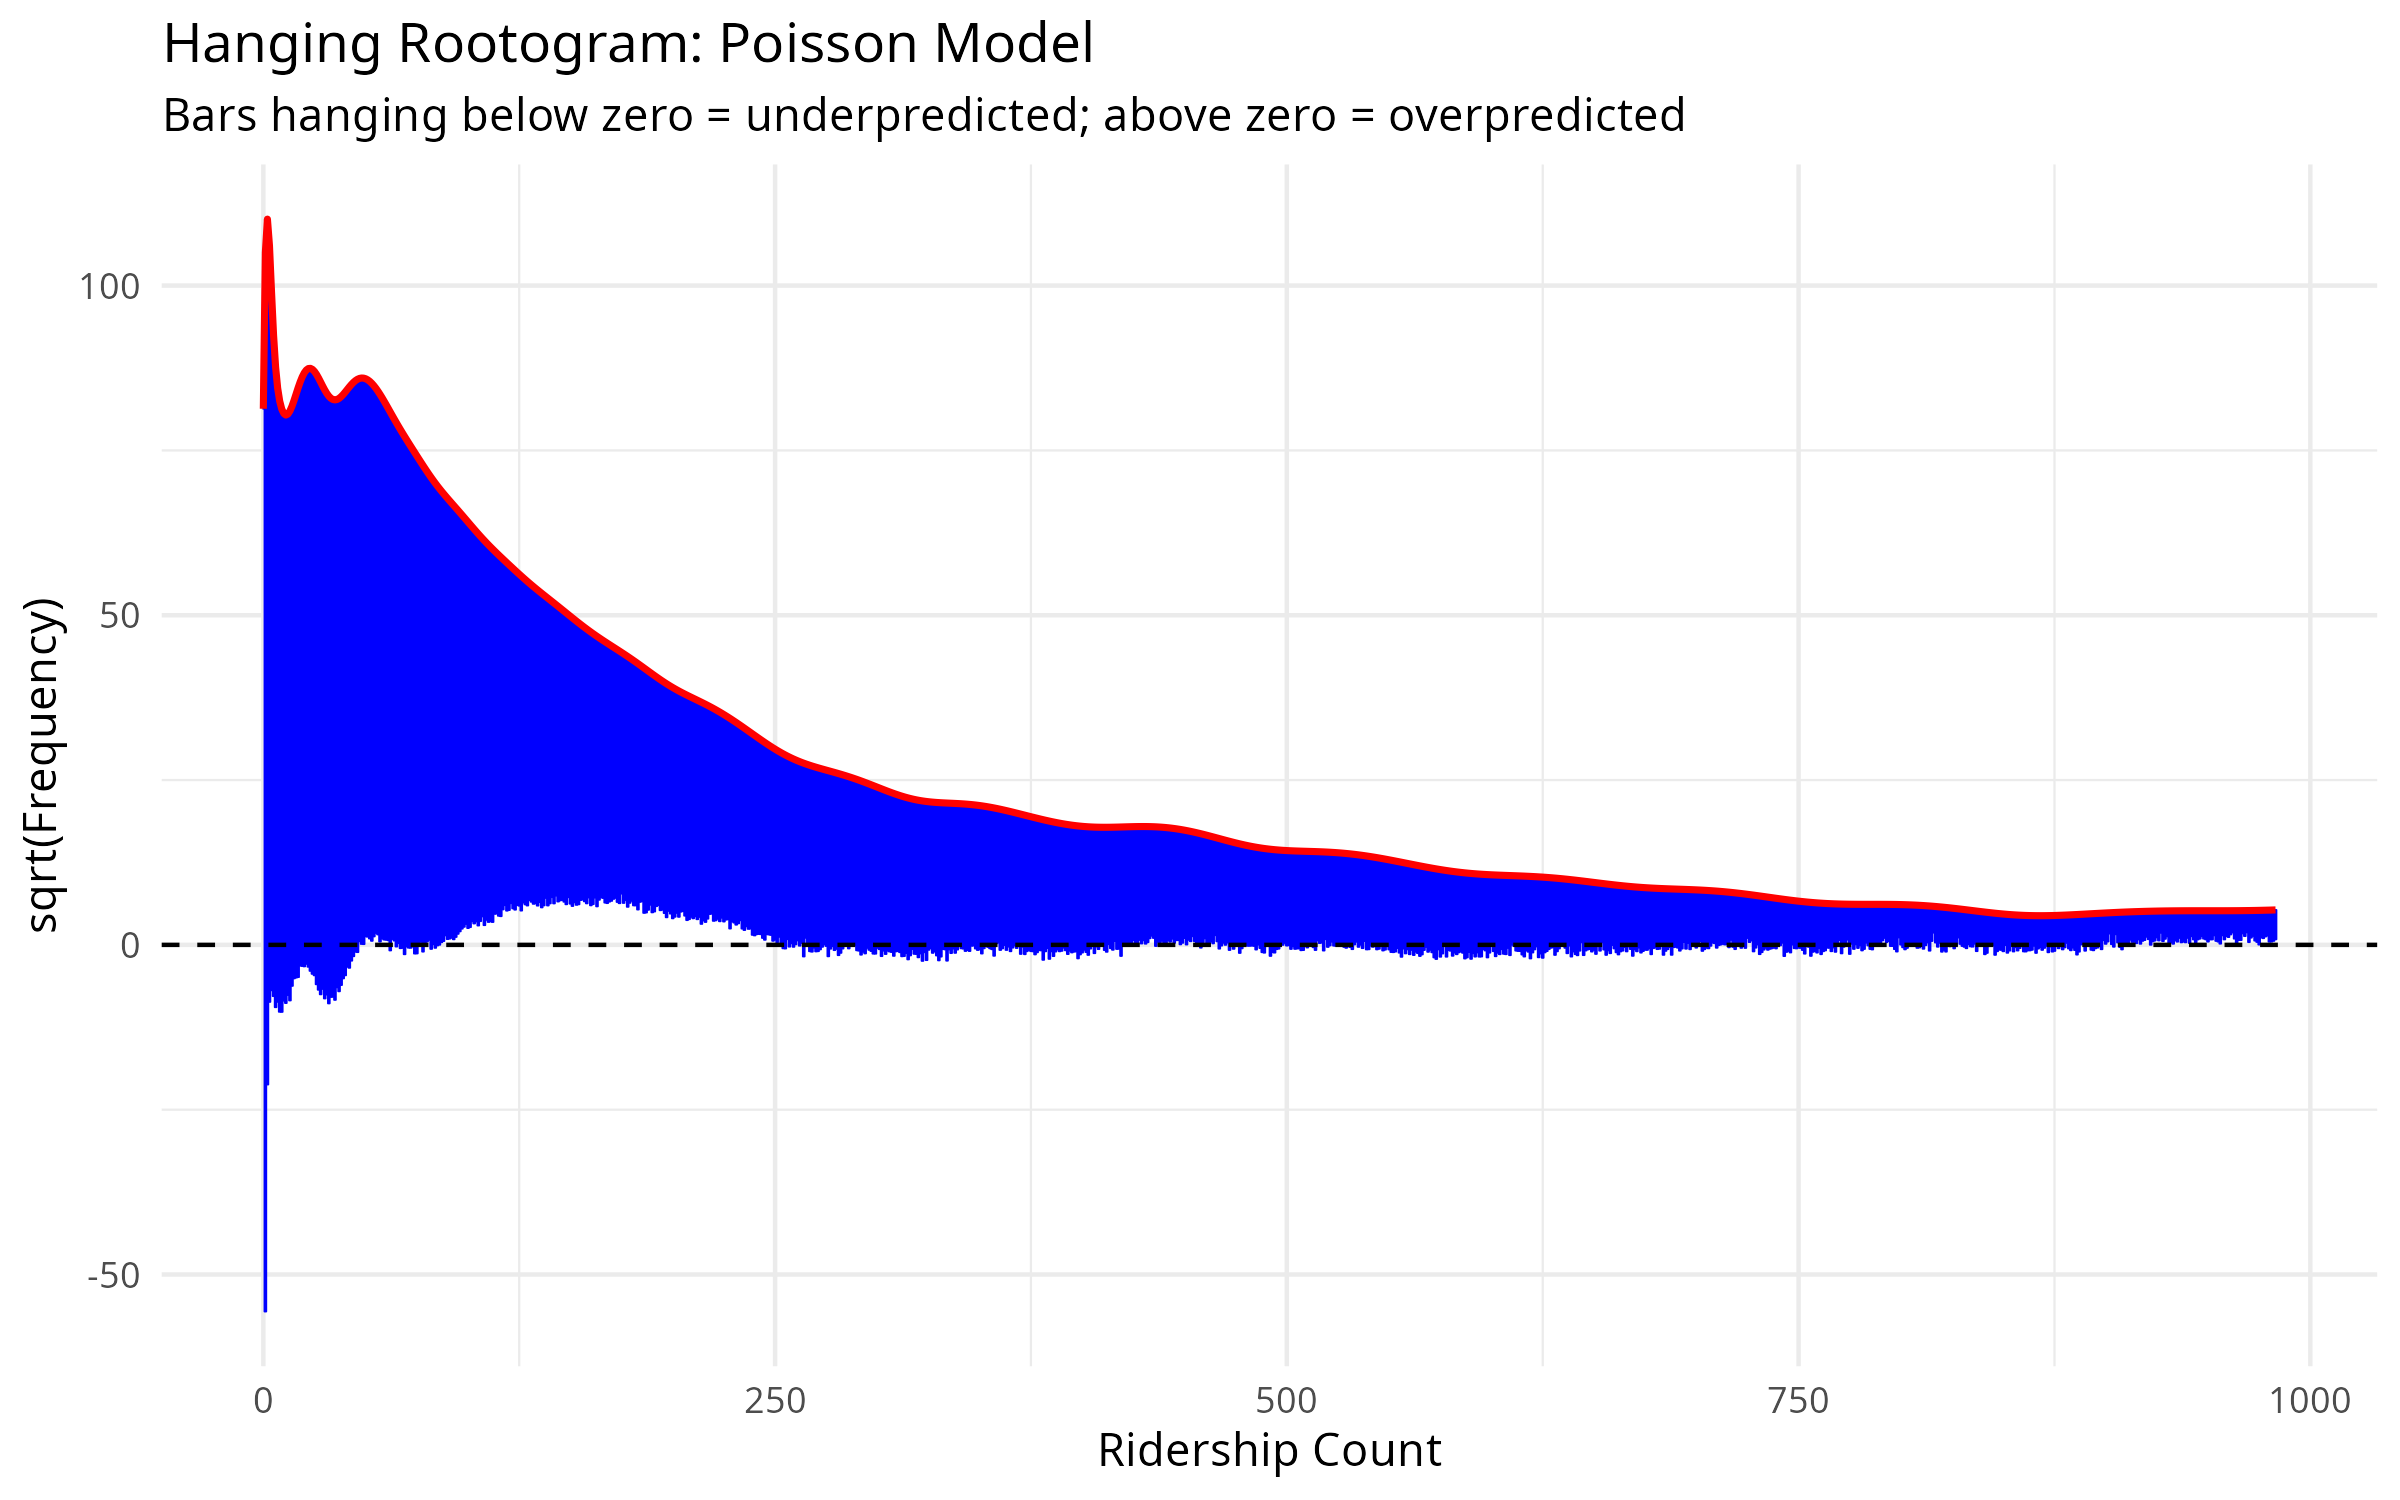
\includegraphics[width=\textwidth]{figs/rootogram_poisson.png}
        \caption{Hanging rootogram of the final Poisson model. Bars below zero
        indicate underprediction; bars above zero indicate overprediction.}
        \label{fig:rootogram}
    \end{subfigure}
    \hfill
    \begin{subfigure}[t]{0.48\textwidth}
        \centering
        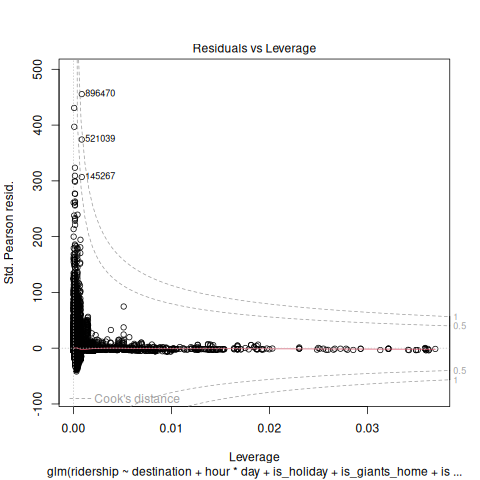
\includegraphics[width=\textwidth]{figs/leverage_residuals_poisson_final.png}
        \caption{Leverage vs.\ standardized residuals. High-residual points
        cluster at low leverage, suggesting missing predictors rather than
        influential observations.}
        \label{fig:leverage}
    \end{subfigure}
    \caption{Diagnostic plots for the final Poisson GLM fitted on the full
    dataset (2023--2025).}
    \label{fig:diagnostics}
\end{figure}

\section{Conclusion}
\label{sec:conclusion}

We conclude that while our model provides a strong baseline for predicting a destination's ridership, some further work is required before adopting this model for use in BART administrative decision making. Our model, when trained on 2023-2024 data and tested on 2025 data, achieved a RMSE of 174, meaning that we expect our estimate of the amount of riders exiting a given station to be off by roughly 174. We believe this amount of error is too high for us to be comfortable using this information for BART planning and that further work will need to be done.

We acknowledge that all of the features we've engineered so far are statistically significant, but further feature engineering may identify gaps in our model that would help predict ridership for a given station. To start, we recommend further inspecting areas/times where the model deviates most from reality and building features to account for this. As an example, our penultimate model identified the hour $\times$ day interaction as a potential gap, so we incorporated it into our final model. After doing this, we also identified some high-residual points clustered around Coliseum on the weekends, which suggests adding a Coliseum $\times$ sports-game or Coliseum $\times$ day interaction to the existing model as a first step for this iterative process.

\newpage

\section{Additional Work}
\label{sec:additional}

\subsection{Model Selection}

For our model selection methodology, we pre-registered the following framework: we'll begin by first conducting feature engineering and using the raw features we've derived. Then, we'll construct the following models based on data from 2023-2024, and select the best model based on whichever achieves the lowest test MSE on the 2025 data. We selected the Basic OLS as a baseline model and opted for various models that account for the right-skewed nature of the ridership. The results are shown below.

\begin{table}[h]
\centering
\begin{tabular}{lrr}
\hline
\textbf{Model} & \textbf{Test MSE} & \textbf{Test RMSE} \\
\hline
Basic OLS LM                             & 41{,}677 & 204 \\
Log-Transformed LM (bias-corrected) & 47{,}682 & 218 \\
\textbf{Poisson GLM}                          & \textbf{32{,}969} & \textbf{182} \\
Negative Binomial GLM                & 46{,}721 & 216 \\
Ridge Poisson ($\lambda = 7.082$)    & 33{,}584 & 183 \\
Ridge NB ($\lambda = 0.599$)         & 43{,}978 & 210 \\
Zero-Inflated NB                     & 46{,}697 & 216 \\
\hline
\end{tabular}
\caption{Test set performance of all preliminary models evaluated. MSE and RMSE are reported on the original ridership scale (riders per station-hour). The Poisson GLM achieves the lowest test MSE and is selected as the final model.}
\label{tab:model_comparison}
\end{table}

For Model 2, the predicted value of the log-transformed model is on the log-scale. However, exponentiating the predicted value will give a biased estimate of the predicted value. Thus, we perform a correction by multiplying by $\exp(\hat{\sigma}^2/2)$ to correct for this bias, though this assumes normality of residuals.

Regarding the selection of $\lambda$ for the ridge regressions, we ran a 5-fold CV using time-based splits for the Poisson Ridge (Model 5). In doing so, we'd technically be using future data (for example, fold 4) to predict past data (for example, fold 3), but we're not currently concerned with autocorrelation. For the NB Ridge (Model 6), we encountered memory issues when trying to perform this procedure, so we instead selected $\lambda$ using a 2023 as our inner-training set and 2024 as our validation set and refit the model on the full training data after selecting $\lambda$.

As previously stated, the Poisson model outperforming the negative binomial model went against our expectations considering the overdispersion. However, this isn't too surprising when considering that the NB model also requires estimating $\theta$ to better model the variance. Although the Poisson model does not correctly capture the variance of the distribution of ridership, it seems that it's still able to predict the conditional mean better.

After performing this analysis, we did a deep dive into where our first Poisson model performed worst and identified weekday peak hours as performing the worst in the model. Table~\ref{tab:stratified_performance} shows that our first Poisson model was unable to identify differences in rush-hour traffic for weekdays vs weekends, which motivated our introduction of the interaction term for the final model. This model achieved a test MSE of $30{,}254$ and test RMSE of 174 prior to being refit on the entire dataset.

\begin{table}[h]
\centering
\begin{tabular}{llrrrr}
\hline
\textbf{Day Type} & \textbf{Period} & \textbf{RMSE} & \textbf{MAE} & \textbf{n} \\
\hline
Weekday & Off-Peak &  84.77 &  39.40 & 197{,}085 \\
Weekend & Off-Peak &  99.59 &  41.21 &  71{,}202 \\
Weekday & PM Peak  & 240.83 & 157.39 &  39{,}109 \\
Weekday & AM Peak  & 444.74 & 170.29 &  38{,}658 \\
Weekend & PM Peak  & 111.55 &  49.33 &  15{,}575 \\
Weekend & AM Peak  & 107.93 &  74.86 &  14{,}465 \\
\hline
\end{tabular}
\caption{Stratified prediction performance of the Poisson GLM (trained on 2023-2024 data, no interaction) by day type and time period. AM Peak covers hours 7--9, PM Peak covers hours 16--18, and Off-Peak covers all remaining hours. RMSE and MAE are on the original ridership scale (riders per station-hour).}
\label{tab:stratified_performance}
\end{table}

\subsection{Model Assumptions}

\subsubsection{Autocorrelation}

Since we are looking at ridership over time, we naturally acknowledge that this problem may be better suited to time-series methods. Naturally, we expect to see seasonality in ridership and dependence between ridership at similar times, which the plots in Figure~\ref{fig:autocorrelation} demonstrate. We attempt to account for this by accounting for the \texttt{day}, \texttt{hour}, and \texttt{season}, but a time-series analysis is likely more robust.

\begin{figure}[h]
    \centering
    \begin{subfigure}[t]{0.48\textwidth}
        \centering
        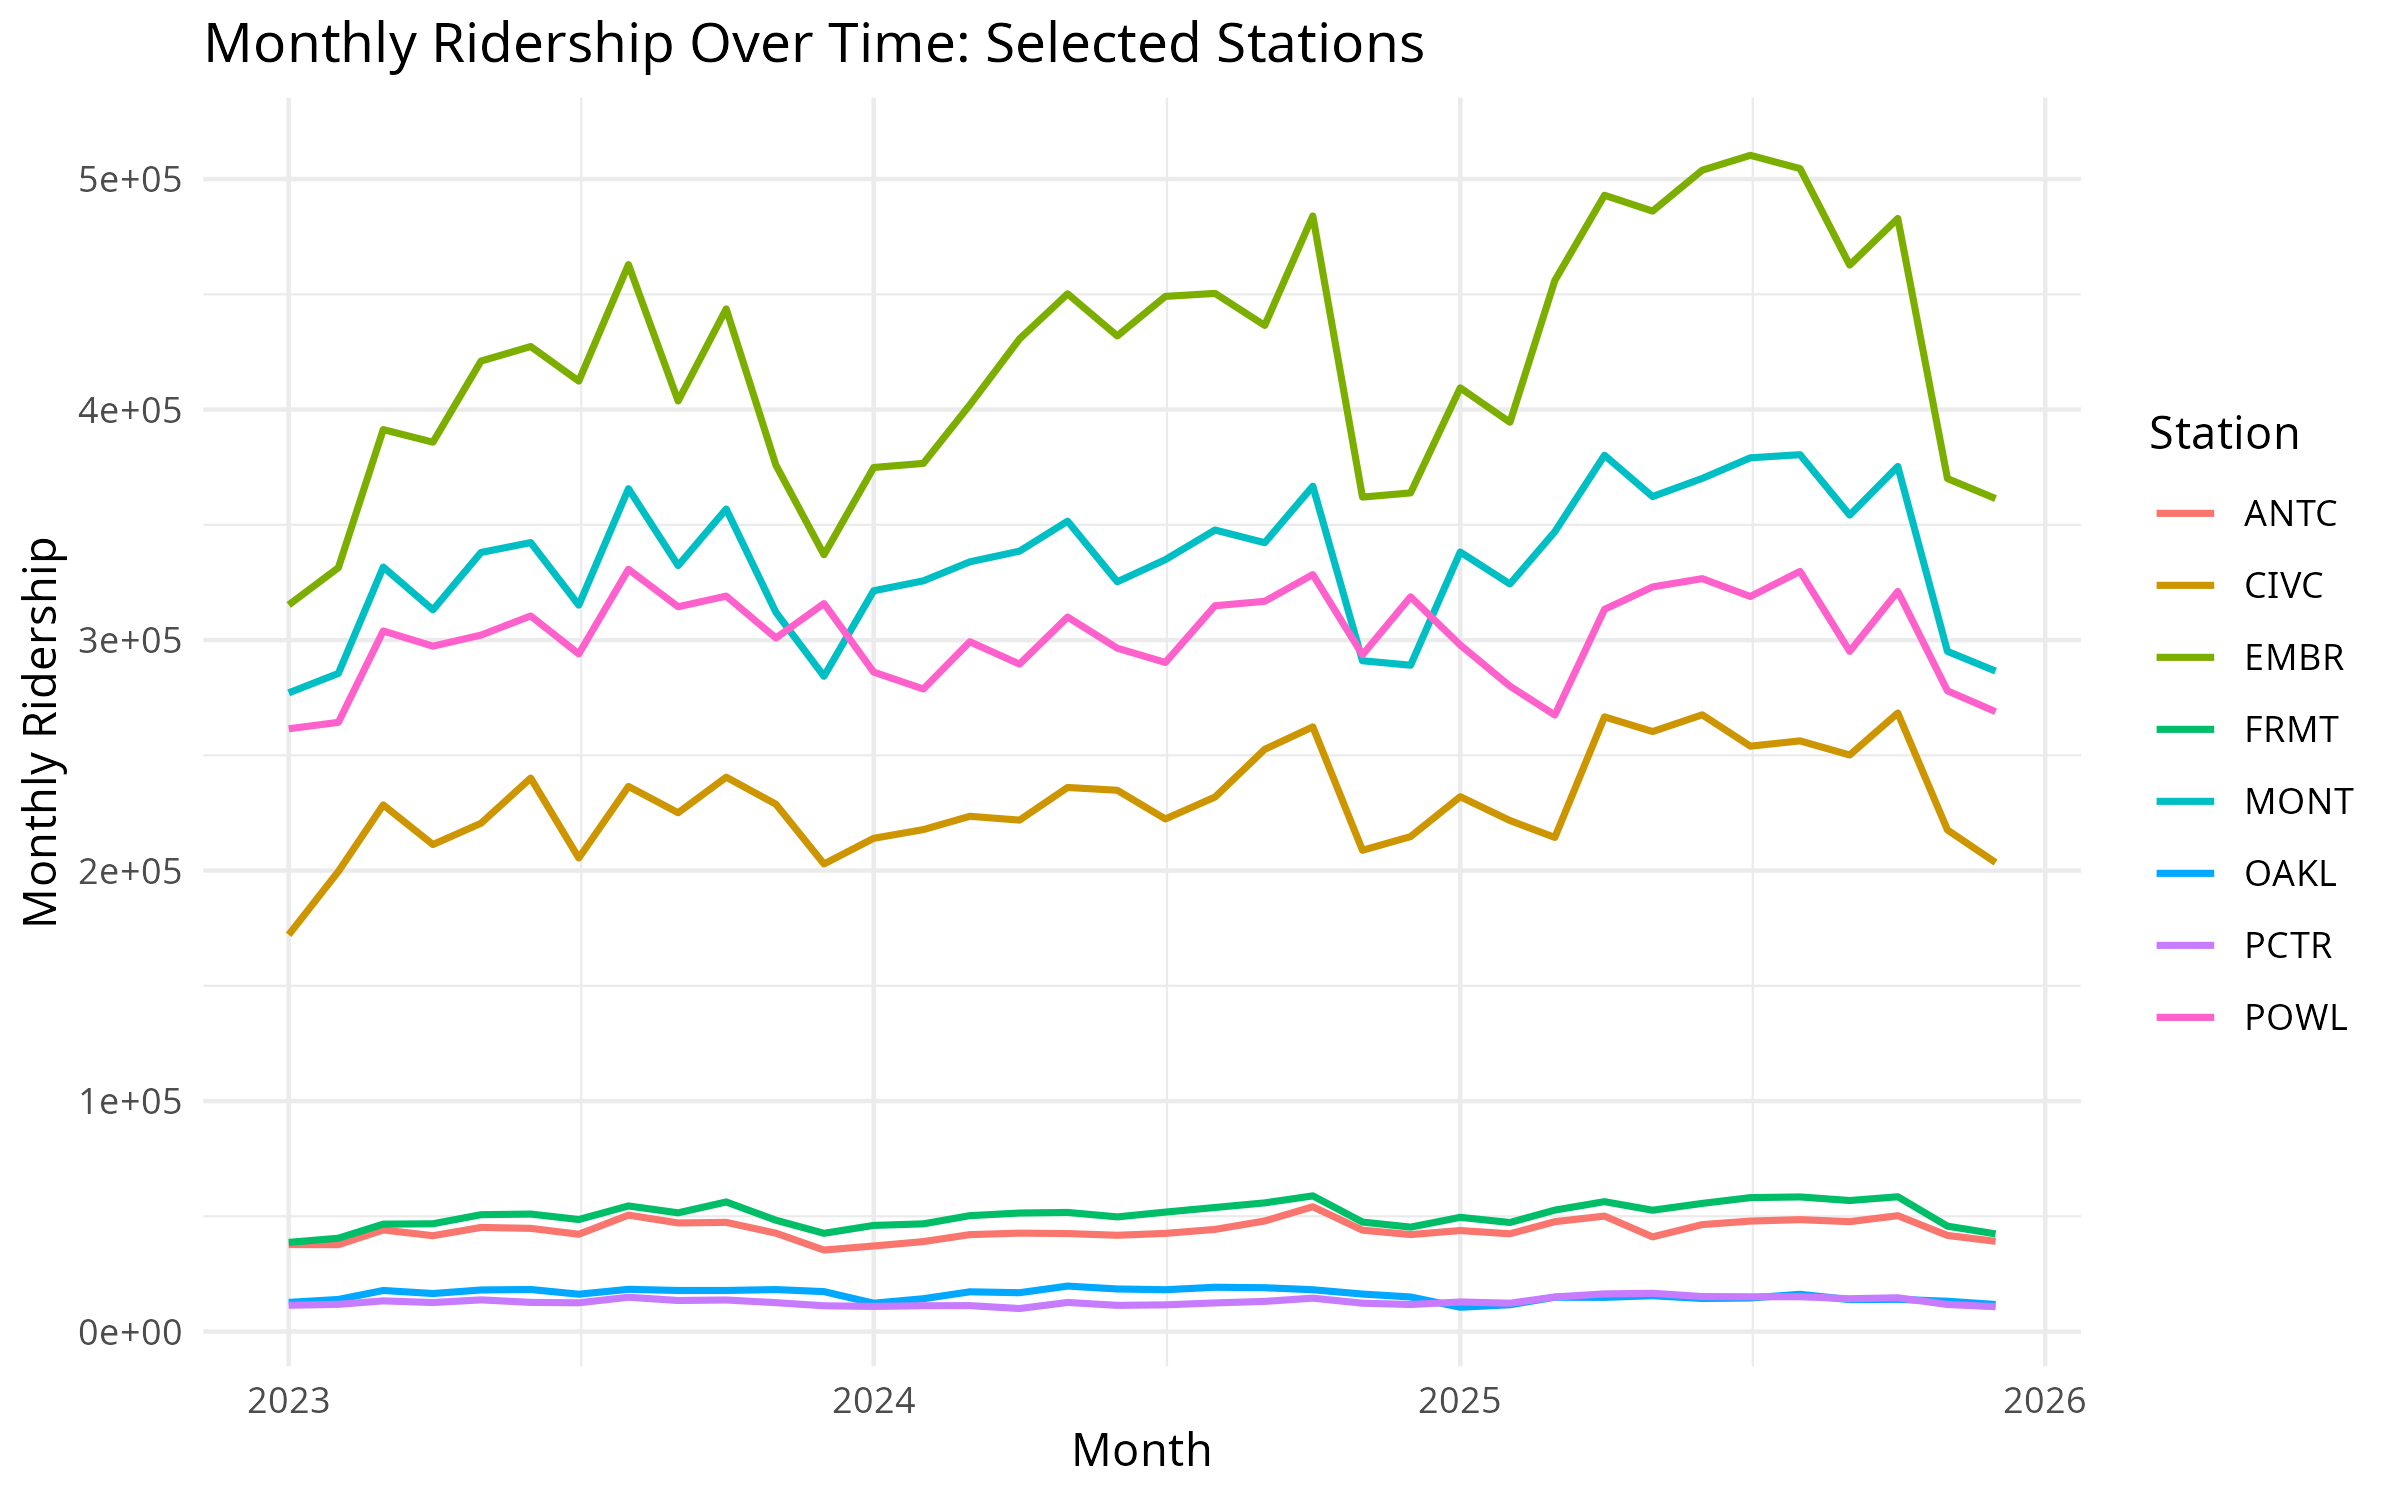
\includegraphics[width=\textwidth]{figs/monthly_ridership.png}
        \caption{Monthly ridership for selected stations. We try to incorporate the overall seasonality by accounting for the season, but our approach likely underfits the true effect.}
        \label{fig:ridership}
    \end{subfigure}
    \hfill
    \begin{subfigure}[t]{0.48\textwidth}
        \centering
        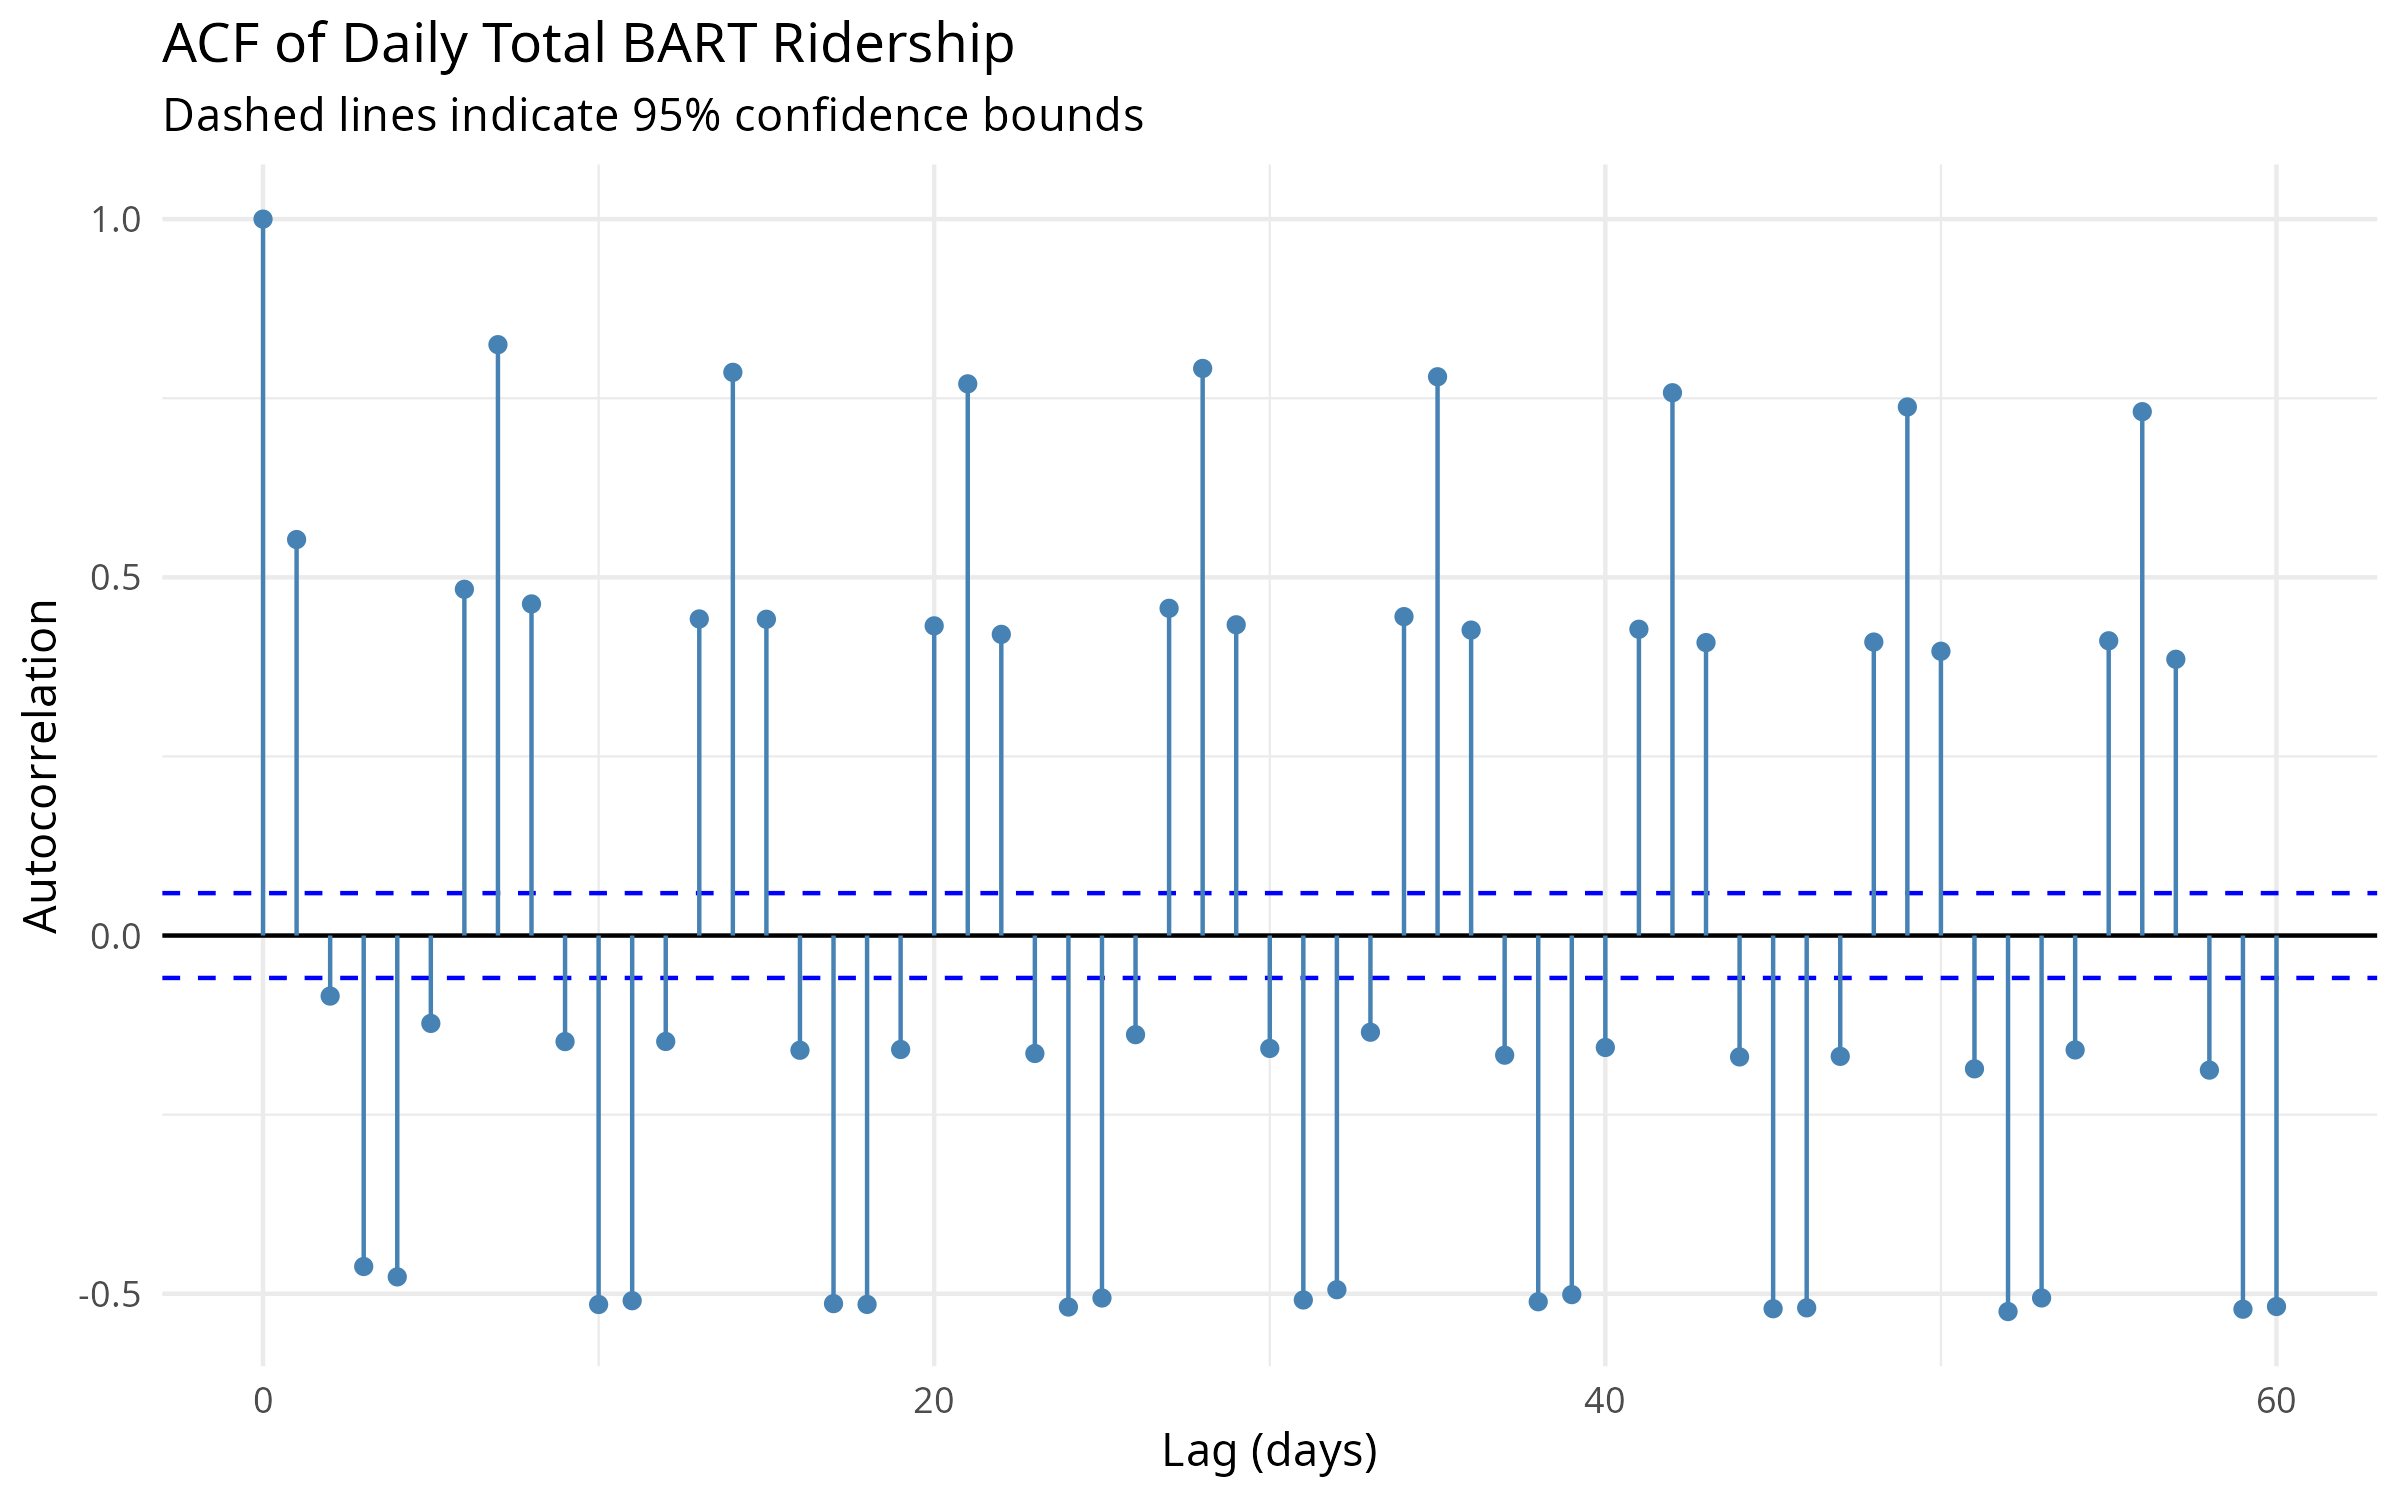
\includegraphics[width=\textwidth]{figs/acf_ridership.png}
        \caption{ACF of overall ridership over days. The highly correlated time lags, especially at multiples of 7 days further demonstrates autocorrelation.}
        \label{fig:acf}
    \end{subfigure}
    \caption{Plots demonstrating that Time Series Analysis may be more appropriate.}
    \label{fig:autocorrelation}
\end{figure}

\subsubsection{Multicollinearity}

We demonstrate multicollinearity via Table~\ref{tab:gvif}. The $\text{GVIF}^{1/2\text{df}}$ for \texttt{hour}, \texttt{day}, and their interaction demonstrate the high collinearity, which is a classical violation of assumptions, but does not present a problem for prediction since future data will reflect the same correlation structure for these variables.

\begin{table}[H]
\centering
\begin{tabular}{lrrr}
\hline
\textbf{Term} & \textbf{GVIF} & \textbf{Df} & \textbf{GVIF\textsuperscript{1/(2$\cdot$Df)}} \\
\hline
Destination        & $1.00 \times 10^{0}$  & 49 & 1.000 \\
Hour               & $8.40 \times 10^{24}$ & 23 & 3.482 \\
Day                & $3.62 \times 10^{3}$  & 2  & 7.758 \\
Holiday            & $1.01 \times 10^{0}$  & 1  & 1.004 \\
Giants Home Game   & $1.21 \times 10^{0}$  & 1  & 1.099 \\
A's Home Game      & $1.17 \times 10^{0}$  & 1  & 1.084 \\
Warriors Home Game & $1.07 \times 10^{0}$  & 1  & 1.034 \\
Season             & $1.47 \times 10^{0}$  & 3  & 1.067 \\
Hour $\times$ Day  & $6.60 \times 10^{27}$ & 46 & 2.006 \\
\hline
\end{tabular}
\caption{Generalized Variance Inflation Factors (GVIF) for the final Poisson GLM.
For terms with more than one degree of freedom, GVIF\textsuperscript{$1/(2 \cdot \text{Df})$}
is the appropriate analog to the square root of VIF and is comparable across terms.
The large GVIF values for \texttt{hour}, \texttt{day}, and their interaction reflect
expected multicollinearity introduced by the interaction term, which is not a concern
for prediction.}
\label{tab:gvif}
\end{table}

\section{Statement of Contribution}
\label{sec:statement}

\begin{itemize}
    \item Drew Galloro worked on the data pulling scripts, data cleaning, exploratory data analysis, and feature engineering.
    \item Benjamin Khothsombath worked on the feature engineering, modeling, and model diagnostics.
\end{itemize}

\section{Appendix}
\label{sec:appendix}

\subsection*{High-Residual Observations}

\begin{table}[h]
\centering
\small
\begin{tabular}{llllrrrr}
\hline
\textbf{Destination} & \textbf{Hour} & \textbf{Day} & \textbf{Holiday} & \textbf{Fitted} & \textbf{Pearson Resid.} & \textbf{Leverage} & \textbf{Abs.\ Resid.} \\
\hline
COLS  & 12 & Sunday   & FALSE & 52.67  & 435.87 & $3.55 \times 10^{-5}$ & 435.87 \\
COLS  & 12 & Sunday   & FALSE & 52.67  & 416.72 & $3.55 \times 10^{-5}$ & 416.72 \\
COLS  & 12 & Sunday   & FALSE & 52.67  & 347.27 & $3.55 \times 10^{-5}$ & 347.27 \\
COLS  & 15 & Saturday & FALSE & 96.03  & 327.47 & $5.82 \times 10^{-5}$ & 327.47 \\
COLS  & 12 & Sunday   & FALSE & 54.38  & 313.34 & $3.70 \times 10^{-5}$ & 313.34 \\
COLS  & 11 & Sunday   & FALSE & 51.63  & 300.66 & $3.49 \times 10^{-5}$ & 300.66 \\
LAKE  & 12 & Saturday & FALSE & 75.46  & 289.46 & $4.53 \times 10^{-5}$ & 289.46 \\
COLS  & 15 & Saturday & FALSE & 96.03  & 286.85 & $5.82 \times 10^{-5}$ & 286.85 \\
COLS  & 12 & Sunday   & FALSE & 52.67  & 252.75 & $3.55 \times 10^{-5}$ & 252.75 \\
16TH  & 11 & Saturday & FALSE & 142.71 & 232.48 & $6.13 \times 10^{-5}$ & 232.48 \\
MLBR  & 1  & Weekday  & TRUE  &  1.72  & 222.19 & $8.67 \times 10^{-6}$ & 222.19 \\
COLS  & 12 & Sunday   & FALSE & 52.67  & 211.27 & $3.55 \times 10^{-5}$ & 211.27 \\
LAKE  & 12 & Saturday & FALSE & 77.91  & 209.15 & $4.56 \times 10^{-5}$ & 209.15 \\
COLS  & 12 & Sunday   & FALSE & 52.67  & 197.77 & $3.55 \times 10^{-5}$ & 197.77 \\
12TH  & 12 & Saturday & FALSE & 120.66 & 192.12 & $5.63 \times 10^{-5}$ & 192.12 \\
LAKE  & 11 & Saturday & FALSE & 76.37  & 189.45 & $4.49 \times 10^{-5}$ & 189.45 \\
LAKE  & 13 & Saturday & FALSE & 78.19  & 186.35 & $4.65 \times 10^{-5}$ & 186.35 \\
MLBR  & 1  & Weekday  & TRUE  &  1.72  & 181.76 & $8.67 \times 10^{-6}$ & 181.76 \\
COLS  & 19 & Saturday & FALSE & 78.25  & 180.74 & $4.83 \times 10^{-5}$ & 180.74 \\
COLS  & 13 & Sunday   & FALSE & 54.57  & 176.98 & $3.65 \times 10^{-5}$ & 176.98 \\
\hline
\end{tabular}
\caption{Top 20 high-residual observations with below-median leverage from the penultimate
Poisson GLM. The concentration of COLS (Coliseum) on weekends suggests an
unmodeled effect, such as a Coliseum $\times$ day or Coliseum $\times$ sports game interaction.}
\label{tab:high_resid}
\end{table}

\newpage
\subsection*{Full Coefficient Table}

\begin{longtable}{lrrrr}
\hline
\textbf{Term} & \textbf{Estimate} & \textbf{Std.\ Error} & \textbf{z value} & \textbf{Pr($>|z|$)} \\
\hline
\endfirsthead
\hline
\textbf{Term} & \textbf{Estimate} & \textbf{Std.\ Error} & \textbf{z value} & \textbf{Pr($>|z|$)} \\
\hline
\endhead
\hline
\endfoot
(Intercept)            &  3.9522 & 0.0020 &  1987.56 & $<2\times10^{-16}$ \\
\hline
\multicolumn{5}{l}{\textit{Destination (reference: 12TH)}} \\
16TH  &  0.1922 & 0.0006 &  299.98 & $<2\times10^{-16}$ \\
19TH  & -0.0346 & 0.0007 &  -51.17 & $<2\times10^{-16}$ \\
24TH  &  0.1513 & 0.0006 &  234.01 & $<2\times10^{-16}$ \\
ANTC  & -1.0238 & 0.0009 & -1106.16 & $<2\times10^{-16}$ \\
ASHB  & -0.8994 & 0.0009 & -1019.49 & $<2\times10^{-16}$ \\
BALB  & -0.2102 & 0.0007 &  -296.47 & $<2\times10^{-16}$ \\
BAYF  & -0.6287 & 0.0008 &  -781.73 & $<2\times10^{-16}$ \\
BERY  & -1.1321 & 0.0010 & -1178.46 & $<2\times10^{-16}$ \\
CAST  & -1.3903 & 0.0011 & -1307.46 & $<2\times10^{-16}$ \\
CIVC  &  0.6189 & 0.0006 &  1052.12 & $<2\times10^{-16}$ \\
COLM  & -1.1146 & 0.0010 & -1167.91 & $<2\times10^{-16}$ \\
COLS  & -0.6051 & 0.0008 &  -758.24 & $<2\times10^{-16}$ \\
CONC  & -0.6560 & 0.0008 &  -808.54 & $<2\times10^{-16}$ \\
DALY  & -0.0282 & 0.0007 &   -41.69 & $<2\times10^{-16}$ \\
DBRK  &  0.1795 & 0.0006 &   279.35 & $<2\times10^{-16}$ \\
DELN  & -0.2575 & 0.0007 &  -358.54 & $<2\times10^{-16}$ \\
DUBL  & -0.4797 & 0.0008 &  -623.66 & $<2\times10^{-16}$ \\
EMBR  &  1.2248 & 0.0005 &  2270.21 & $<2\times10^{-16}$ \\
FRMT  & -0.8920 & 0.0009 & -1013.40 & $<2\times10^{-16}$ \\
FTVL  & -0.2195 & 0.0007 &  -308.74 & $<2\times10^{-16}$ \\
GLEN  & -0.4301 & 0.0008 &  -569.27 & $<2\times10^{-16}$ \\
HAYW  & -0.8022 & 0.0009 &  -940.73 & $<2\times10^{-16}$ \\
LAFY  & -1.1422 & 0.0010 & -1184.31 & $<2\times10^{-16}$ \\
LAKE  & -0.4659 & 0.0008 &  -609.80 & $<2\times10^{-16}$ \\
MCAR  & -0.2678 & 0.0007 &  -371.60 & $<2\times10^{-16}$ \\
MLBR  & -0.8806 & 0.0009 & -1002.63 & $<2\times10^{-16}$ \\
MLPT  & -1.3431 & 0.0010 & -1287.78 & $<2\times10^{-16}$ \\
MONT  &  0.9936 & 0.0006 &  1789.51 & $<2\times10^{-16}$ \\
NBRK  & -1.0082 & 0.0009 & -1098.94 & $<2\times10^{-16}$ \\
NCON  & -2.0760 & 0.0014 & -1460.39 & $<2\times10^{-16}$ \\
OAKL  & -2.0323 & 0.0014 & -1447.50 & $<2\times10^{-16}$ \\
ORIN  & -1.3910 & 0.0011 & -1307.17 & $<2\times10^{-16}$ \\
PCTR  & -2.2464 & 0.0015 & -1459.58 & $<2\times10^{-16}$ \\
PHIL  & -0.7337 & 0.0008 &  -881.05 & $<2\times10^{-16}$ \\
PITT  & -0.8853 & 0.0009 & -1008.14 & $<2\times10^{-16}$ \\
PLZA  & -0.8437 & 0.0009 &  -975.44 & $<2\times10^{-16}$ \\
POWL  &  0.8918 & 0.0006 &  1583.57 & $<2\times10^{-16}$ \\
RICH  & -0.7302 & 0.0008 &  -875.64 & $<2\times10^{-16}$ \\
ROCK  & -0.6359 & 0.0008 &  -788.73 & $<2\times10^{-16}$ \\
SANL  & -0.4138 & 0.0008 &  -550.40 & $<2\times10^{-16}$ \\
SBRN  & -1.1686 & 0.0010 & -1199.50 & $<2\times10^{-16}$ \\
SFIA  & -0.0910 & 0.0007 &  -132.52 & $<2\times10^{-16}$ \\
SHAY  & -1.2685 & 0.0010 & -1252.07 & $<2\times10^{-16}$ \\
SSAN  & -1.2774 & 0.0010 & -1256.37 & $<2\times10^{-16}$ \\
UCTY  & -0.9818 & 0.0009 & -1079.83 & $<2\times10^{-16}$ \\
WARM  & -1.4570 & 0.0011 & -1334.73 & $<2\times10^{-16}$ \\
WCRK  & -0.5644 & 0.0008 &  -716.69 & $<2\times10^{-16}$ \\
WDUB  & -1.3458 & 0.0010 & -1285.03 & $<2\times10^{-16}$ \\
WOAK  & -0.3217 & 0.0007 &  -439.64 & $<2\times10^{-16}$ \\
\hline
\multicolumn{5}{l}{\textit{Hour (reference: hour 0)}} \\
Hour 1  & -1.5595 & 0.0048 &  -325.39 & $<2\times10^{-16}$ \\
Hour 2  & -2.2304 & 0.0210 &  -106.37 & $<2\times10^{-16}$ \\
Hour 3  & -3.2591 & 0.0532 &   -61.28 & $<2\times10^{-16}$ \\
Hour 4  & -2.9188 & 0.0391 &   -74.73 & $<2\times10^{-16}$ \\
Hour 5  & -2.9519 & 0.0119 &  -248.69 & $<2\times10^{-16}$ \\
Hour 6  & -0.3479 & 0.0030 &  -115.16 & $<2\times10^{-16}$ \\
Hour 7  &  0.3925 & 0.0025 &   157.63 & $<2\times10^{-16}$ \\
Hour 8  &  0.7744 & 0.0023 &   332.92 & $<2\times10^{-16}$ \\
Hour 9  &  0.9804 & 0.0023 &   434.36 & $<2\times10^{-16}$ \\
Hour 10 &  1.1217 & 0.0022 &   506.10 & $<2\times10^{-16}$ \\
Hour 11 &  1.2760 & 0.0022 &   586.03 & $<2\times10^{-16}$ \\
Hour 12 &  1.3695 & 0.0022 &   635.18 & $<2\times10^{-16}$ \\
Hour 13 &  1.3726 & 0.0022 &   636.79 & $<2\times10^{-16}$ \\
Hour 14 &  1.3831 & 0.0022 &   642.34 & $<2\times10^{-16}$ \\
Hour 15 &  1.4149 & 0.0021 &   659.13 & $<2\times10^{-16}$ \\
Hour 16 &  1.4981 & 0.0021 &   703.37 & $<2\times10^{-16}$ \\
Hour 17 &  1.5214 & 0.0021 &   715.82 & $<2\times10^{-16}$ \\
Hour 18 &  1.4319 & 0.0021 &   668.15 & $<2\times10^{-16}$ \\
Hour 19 &  1.1915 & 0.0022 &   542.07 & $<2\times10^{-16}$ \\
Hour 20 &  0.8927 & 0.0023 &   390.63 & $<2\times10^{-16}$ \\
Hour 21 &  0.7826 & 0.0023 &   336.82 & $<2\times10^{-16}$ \\
Hour 22 &  0.6841 & 0.0024 &   289.76 & $<2\times10^{-16}$ \\
Hour 23 &  0.4839 & 0.0024 &   197.77 & $<2\times10^{-16}$ \\
\hline
\multicolumn{5}{l}{\textit{Day (reference: Saturday)}} \\
Sunday  & -0.0832 & 0.0028 &  -29.99 & $<2\times10^{-16}$ \\
Weekday & -0.5872 & 0.0023 & -260.79 & $<2\times10^{-16}$ \\
\hline
\multicolumn{5}{l}{\textit{Other predictors}} \\
Holiday (TRUE)        & -0.6962 & 0.0006 & -1120.69 & $<2\times10^{-16}$ \\
Giants Home (TRUE)    &  0.0311 & 0.0002 &   156.49 & $<2\times10^{-16}$ \\
A's Home (TRUE)       &  0.0076 & 0.0002 &    38.77 & $<2\times10^{-16}$ \\
Warriors Home (TRUE)  & -0.0209 & 0.0003 &   -75.24 & $<2\times10^{-16}$ \\
Season: Spring        & -0.0597 & 0.0002 &  -247.49 & $<2\times10^{-16}$ \\
Season: Summer        & -0.0313 & 0.0002 &  -132.15 & $<2\times10^{-16}$ \\
Season: Winter        & -0.1389 & 0.0002 &  -588.60 & $<2\times10^{-16}$ \\
\hline
\multicolumn{5}{l}{\textit{Hour $\times$ Sunday interaction (reference: hour 0 $\times$ Saturday)}} \\
Hour 1  $\times$ Sun  &  0.0043 & 0.0069 &    0.62 & 0.533 \\
Hour 2  $\times$ Sun  &  0.7086 & 0.0267 &   26.55 & $<2\times10^{-16}$ \\
Hour 3  $\times$ Sun  &  0.8416 & 0.0729 &   11.55 & $<2\times10^{-16}$ \\
Hour 4  $\times$ Sun  & -0.9741 & 0.1124 &   -8.66 & $<2\times10^{-16}$ \\
Hour 5  $\times$ Sun  & -0.7551 & 0.0439 &  -17.21 & $<2\times10^{-16}$ \\
Hour 6  $\times$ Sun  & -2.8156 & 0.0279 & -101.04 & $<2\times10^{-16}$ \\
Hour 7  $\times$ Sun  & -2.0558 & 0.0062 & -332.99 & $<2\times10^{-16}$ \\
Hour 8  $\times$ Sun  & -0.2628 & 0.0034 &  -76.36 & $<2\times10^{-16}$ \\
Hour 9  $\times$ Sun  & -0.0918 & 0.0033 &  -28.05 & $<2\times10^{-16}$ \\
Hour 10 $\times$ Sun  & -0.0517 & 0.0032 &  -16.12 & $<2\times10^{-16}$ \\
Hour 11 $\times$ Sun  & -0.0530 & 0.0031 &  -16.84 & $<2\times10^{-16}$ \\
Hour 12 $\times$ Sun  & -0.0753 & 0.0031 &  -24.15 & $<2\times10^{-16}$ \\
Hour 13 $\times$ Sun  & -0.0958 & 0.0031 &  -30.67 & $<2\times10^{-16}$ \\
Hour 14 $\times$ Sun  & -0.1384 & 0.0031 &  -44.29 & $<2\times10^{-16}$ \\
Hour 15 $\times$ Sun  & -0.1739 & 0.0031 &  -55.71 & $<2\times10^{-16}$ \\
Hour 16 $\times$ Sun  & -0.1615 & 0.0031 &  -52.21 & $<2\times10^{-16}$ \\
Hour 17 $\times$ Sun  & -0.1665 & 0.0031 &  -53.92 & $<2\times10^{-16}$ \\
Hour 18 $\times$ Sun  & -0.2214 & 0.0031 &  -70.85 & $<2\times10^{-16}$ \\
Hour 19 $\times$ Sun  & -0.2373 & 0.0032 &  -73.75 & $<2\times10^{-16}$ \\
Hour 20 $\times$ Sun  & -0.2015 & 0.0033 &  -60.19 & $<2\times10^{-16}$ \\
Hour 21 $\times$ Sun  & -0.2457 & 0.0034 &  -71.78 & $<2\times10^{-16}$ \\
Hour 22 $\times$ Sun  & -0.3708 & 0.0035 & -104.99 & $<2\times10^{-16}$ \\
Hour 23 $\times$ Sun  & -0.4939 & 0.0037 & -132.00 & $<2\times10^{-16}$ \\
\hline
\multicolumn{5}{l}{\textit{Hour $\times$ Weekday interaction (reference: hour 0 $\times$ Saturday)}} \\
Hour 1  $\times$ Wkdy &  0.1327 & 0.0056 &   23.70 & $<2\times10^{-16}$ \\
Hour 2  $\times$ Wkdy &  0.7375 & 0.0231 &   31.95 & $<2\times10^{-16}$ \\
Hour 3  $\times$ Wkdy &  1.3586 & 0.0542 &   25.08 & $<2\times10^{-16}$ \\
Hour 4  $\times$ Wkdy &  1.0376 & 0.0393 &   26.39 & $<2\times10^{-16}$ \\
Hour 5  $\times$ Wkdy &  3.7314 & 0.0120 &  312.16 & $<2\times10^{-16}$ \\
Hour 6  $\times$ Wkdy &  2.2338 & 0.0033 &  683.17 & $<2\times10^{-16}$ \\
Hour 7  $\times$ Wkdy &  2.2004 & 0.0028 &  795.13 & $<2\times10^{-16}$ \\
Hour 8  $\times$ Wkdy &  2.1540 & 0.0026 &  823.61 & $<2\times10^{-16}$ \\
Hour 9  $\times$ Wkdy &  1.5990 & 0.0026 &  624.56 & $<2\times10^{-16}$ \\
Hour 10 $\times$ Wkdy &  0.9190 & 0.0025 &  362.00 & $<2\times10^{-16}$ \\
Hour 11 $\times$ Wkdy &  0.5756 & 0.0025 &  229.15 & $<2\times10^{-16}$ \\
Hour 12 $\times$ Wkdy &  0.4765 & 0.0025 &  191.05 & $<2\times10^{-16}$ \\
Hour 13 $\times$ Wkdy &  0.5261 & 0.0025 &  211.20 & $<2\times10^{-16}$ \\
Hour 14 $\times$ Wkdy &  0.6680 & 0.0025 &  268.99 & $<2\times10^{-16}$ \\
Hour 15 $\times$ Wkdy &  0.9285 & 0.0025 &  376.10 & $<2\times10^{-16}$ \\
Hour 16 $\times$ Wkdy &  1.2273 & 0.0024 &  501.79 & $<2\times10^{-16}$ \\
Hour 17 $\times$ Wkdy &  1.4921 & 0.0024 &  612.22 & $<2\times10^{-16}$ \\
Hour 18 $\times$ Wkdy &  1.3096 & 0.0025 &  533.01 & $<2\times10^{-16}$ \\
Hour 19 $\times$ Wkdy &  0.9283 & 0.0025 &  368.37 & $<2\times10^{-16}$ \\
Hour 20 $\times$ Wkdy &  0.7067 & 0.0026 &  269.98 & $<2\times10^{-16}$ \\
Hour 21 $\times$ Wkdy &  0.5787 & 0.0027 &  217.13 & $<2\times10^{-16}$ \\
Hour 22 $\times$ Wkdy &  0.5519 & 0.0027 &  203.93 & $<2\times10^{-16}$ \\
Hour 23 $\times$ Wkdy &  0.4332 & 0.0028 &  154.28 & $<2\times10^{-16}$ \\
\hline
\caption{Full coefficient table for the final Poisson GLM. All coefficients are on the log-rate scale. The single non-significant coefficient is Hour~1~$\times$~Sunday ($p = 0.533$). Reference levels are: 12TH for destination, hour~0 for hour, and Saturday for day.}
\label{tab:full_coefs}
\end{longtable}

\end{document}
